\usepackage{graphicx} % Required for inserting images

\title{Assignment 6: Using the Nagel-Schreckenberg model to investigate traffic patterns on the R44 in Stellenbosch}
\author{Zander Vermeulen}
\date{13 November 2023}

\begin{document}

\maketitle

\section*{Introduction}

The aim of this project was to adapt and expand the model proposed in (Nagel \& Schrekenberg, 1992) to model traffic flow (specifically, southbound traffic during evening peak hours) on and around the R44 between Merriman avenue and the Y-junction with the R310. Data from Google Maps as well as the author's personal experience shows that this is one of the most congested road segments in Stellenbosch (fig. 1). This model could then be used to evaluate strategies employed by road users in an attempt to circumvent this traffic, as well as considering infrastructure changes that could ameliorate the situation.

This project proceeded in multiple phases. At first, the original Nagel-Schreckenberg model was only slightly adjusted to model a linear road segment. Phase 2 involved the addition of junctions along this road segment, while phase 3 considered the effects of traffic lights. In phase 4, the strategy of using Du Toit street to bypass traffic was evaluated, and phase 5 examined the effects that having multiple lanes has on traffic flow, as well as the effects of adding/removing lanes.

\begin{figure}
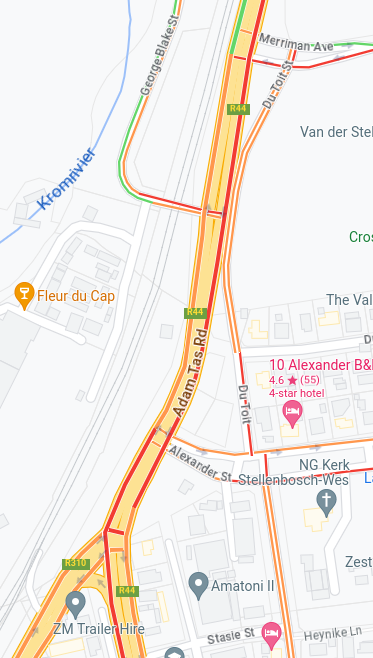
\includegraphics[scale = 0.75]{images/road.png}
\caption{\label{fig} The roads in question. Red shading indicated the slowest traffic, whereas green indicates the fastest. Data shows typical traffic on a Monday evening at 5 pm. Image credit: (Google, 2023)}
\end{figure}

\section*{Phase 1: Simple model on a linear road segment}

\subsection*{The model}

For phase 1, the model stuck closely to the original proposal in (Nagel \& Schrekenberg, 1992), albeit with different boundary conditions that better reflect the reality of the road in question. In this model, a vehicle appears at the start(north) end of the road with a certain probability $q$ (provided the first cell is unoccupied). $p$ and $v$ have the same interpretation as in the original model, ie. the probability of a vehicle randomly decelerating and the top speed for all vehicles respectively. The final variable is the length of the road $l$, in cells. The main observable of interest is the number of time-steps a vehicle spends on the road, on average.

\subsection*{Implementation}

\subsection*{Results}

\subsection*{Discussion}

\section*{Conclusion}

\section*{References}

%TODO fix alignment of references here

Nagel, K.; Schreckenberg, M. (1992). "A cellular automaton model for freeway traffic". \textit{Journal de Physique I} 2(12) doi:10.1051/jp1:1992277

Google. (2023). Retrieved 25 October 2023 from https://www.google.com/maps/@-33.9354554,18.8545061,17z/data=!5m1!1e1?entry=ttu

\end{document}